\documentclass[mathserif,blue]{beamer}
\usepackage[includemp=true,marginparsep=.5cm,marginparwidth=3cm,left=.7cm,right=1.7cm,top=2cm,bottom=1.5cm]{geometry}
\usepackage{amsmath,amssymb}
\usepackage{stmaryrd}
\usepackage{verbatim}
\usepackage{mdwlist}%提供紧凑的列表
\usepackage{graphicx}
\usepackage{tikz}
\usepackage{ifthen}
\usepackage[colorlinks=true,linkcolor=blue,citecolor=blue]{hyperref}
\usepackage{xfrac}%提供斜分数命令,\sfrac{1}{3}
\usepackage{ctex}
%\usepackage{titlesec}%标题格式
\usepackage{fancyhdr}%页眉页脚
\usepackage{listings}%插入代码
\usepackage{framed}
\usepackage{lipsum}
\usepackage{subfig}%子图
\usepackage{tabularx,booktabs}%插入表格
\usepackage{indentfirst} %首行缩进
\usepackage{array} 
\usepackage{longtable}%长表格
\usepackage{multirow}%使用多栏宏包
\usepackage{wrapfig}%文字环绕
\usepackage{extarrows}
\usepackage{ulem,bm}
\usepackage{cite}%参考文献
\usepackage[super,square,comma,sort&compress]{natbib} 
\usepackage{setspace}%设定行距

\setCJKfamilyfont{huawen}{STXihei}
\setCJKfamilyfont{hwzhs}{STZhongsong}
\newcommand\xihei{\CJKfamily{huawen}} %华文细黑
\newcommand\zhongsong{\CJKfamily{hwzhs}}%华文中宋
\usetikzlibrary{arrows,arrows.spaced,arrows.meta,calc,intersections,through,backgrounds,math,angles,shapes}

\newtheorem{theorem}{定理}
\newtheorem{definition}{\hei 定义}
\newtheorem{property}{问题}
\newtheorem{proposition}{猜测}
\newtheorem{lemma}{引理}
\newtheorem{corollary}{推论}

\newcommand\Dd{\displaystyle}\newcommand{\Tt}{\textstyle}\newcommand{\Ss}{\scriptstyle}\newcommand{\Sss}{\scriptscriptstyle}%
\setlength\mathsurround{0.5ex}%数学模式与文本模式混排时留出的间距
\newcommand\an[1][a]{\ensuremath{\{#1_n\}}}%sequence
\newcommand\ud{\mathrm{d}}
\newcommand{\ue}{\mathrm{e}}%正体字母
\newcommand\triabc{\ensuremath{\triangle ABC}}%三角形ABC
\newcommand\cnm[2][n]{\ensuremath{\textrm{C}^{#2}_{#1}}}%组合数
%数学题目编辑
\newcommand\lines[1][1.2]{\,\underline{\mbox{\hspace{#1cm}}}\,}% 填空题的横线
\newcommand\brackets[1][2]{\nolinebreak\hfill\mbox{~(\hspace{#1em})}\\}% 选择题的括号
%扩展命令
\newcommand\qqquad{\qquad\quad}
\def\aside#1{\marginpar{\footnotesize #1}}
%自动编号之最简
\newcommand\numa{\refstepcounter{numi}\thenumi}\newcounter{numi}
\newcommand\numb{\refstepcounter{numii}\thenumii}\newcounter{numii}
\newcommand\numc{\refstepcounter{numiii}\thenumiii}\newcounter{numiii}
\newcommand\numaa{\refstepcounter{numai}\thenumai}\newcounter{numai}[numi]

\newcommand{\question}[1][]{\par\vspace{1ex}\noindent\refstepcounter{numberi}\textbf{\thenumberi.}\ensuremath{#1}}\newcounter{numberi}[subsection]% 每道小题自动编号
\newcommand\quson{\\ \hspace*{1em}\refstepcounter{numberii}\thenumberii)~}\newcounter{numberii}[numberi]% 每道小题自动编号
\newcommand\choice[5][4]{\vspace*{-1em}\begin{tasks}(#1)\task$#2$\task$#3$\task$#4$\task$#5$\end{tasks}\vspace*{-1.2em}}%选择题排版之数学模式
\newcommand\choicex[5][4]{\vspace*{-1em}\begin{tasks}(#1)\task#2\task#3\task#4\task#5\end{tasks}\vspace*{-1.2em}}%选择题排版之数学模式
\newcommand\tbs[1][]{\texttt{\char92#1}}
\newcommand\bpics[1]{\par\vspace{1ex}\noindent\begin{minipage}{\textwidth}\begin{minipage}{#1\textwidth}}
\newcommand\mpics[1]{\end{minipage}\begin{minipage}{#1\textwidth}\linespread{1}}
\newcommand\epics{\end{minipage}\end{minipage}\par\vspace{2ex}}

\newcommand\set[1]{\lbrace\ensuremath{#1}\rbrace}
\newcommand\setx[1]{\{#1\}}

\newcommand\mybf[1]{{\bm#1}}
\def\bfR{\mybf R}
\def\bfN{\mybf N}
\def\bfZ{\mybf Z}
\def\bfQ{\mybf Q}
\def\bfC{\mybf C}
\def\bfZp{\mybf Z^+}

\newcommand\myvec[1]{\bm#1}
\def\veca{\myvec a}
\def\vecb{\myvec b}
\def\vecc{\myvec c}
\def\vecd{\myvec d}
\def\vece{\myvec e}
\def\vecf{\myvec f}
\def\vecs{\myvec e}
\def\vecp{\myvec p}
\def\vecq{\myvec q}
\def\veci{\myvec i}
\def\vecj{\myvec j}
\def\vecei{\myvec{e_1}}
\def\veceii{\myvec{e_2}}
\def\veczero{\myvec 0}
\newcommand\lvec[1]{\overrightarrow{#1}}
%background rectangle/.style={draw=blue!50,fill=blue!20,rounded corners=1ex},show background rectangle

%\begin{columns}\begin{column}{\.5\textwidth} \end{column}\begin{column}{.5\textwidth} \end{column}\end{columns}

%受命于tikz
\def\mystyle{\tikzset{myvec/.style={-stealth}}}
%兼容于beamer
\def\pause{}

%%%listings设置    \begin{lstlisting} !!code!! \end{lstlisting}
\lstset{
        numbers=none, %设置行号位置
       numberstyle=\wuhao, %设置行号大小
        keywordstyle=\color{blue}, %设置关键字颜色
        commentstyle=\color[cmyk]{1,0,1,0}, %设置注释颜色
        %frame=shadowbox, %设置边框格式
        escapeinside=``, %逃逸字符(1左面的键),用于显示中文
        breaklines, %自动折行
        extendedchars=false, %解决代码跨页时,章节标题,页眉等汉字不显示的问题
        xleftmargin=0em,xrightmargin=0em, aboveskip=0.5em,%设置边距
        framextopmargin=0pt,framexbottommargin=2pt,abovecaptionskip=-3pt,
        belowcaptionskip=0pt,  
        %tabsize=1, %设置tab空格数
        showspaces=false %不显示空格
        commentstyle=\color{red!50!green!50!blue!50},%浅灰色的注释  
        keywordstyle=\color{blue!90}\bfseries, %代码关键字的颜色为蓝色,粗体  
        rulesepcolor=\color{red!20!green!20!blue!20},%代码块边框为淡青色  
        numberstyle={\color[RGB]{255,1,1}\scriptsize} ,%设置行号的大小,大小有tiny,scriptsize,footnotesize,small,normalsize,large等  
        numbersep=8pt,  %设置行号与代码的距离,默认是5pt  
  basicstyle=\footnotesize, % 这句设置代码的大小  
        frame=shadowbox, %把代码用带有阴影的框圈起来  
        backgroundcolor=\color[RGB]{245,245,244},   %代码背景色         
       }
%\usepackage[includemp=true,marginparsep=.5cm,marginparwidth=3cm,left=2.5cm,right=2cm]{geometry}%带有旁注marginpar
%\usepackage[paperheight=6in,paperwidth=4.5in,margin=1cm]{geometry}%kindel专用


\begin{document}
\mytitle{向量的减法}
%这节课我们要学习的正如大屏幕上显示的---向量的减法
%当你学习一件新东西的时候,先想一想你已经会了什么。

\begin{frame}{学习目标}
    \begin{enumerate}
      \item 记住向量减法的定义
      \item 会作两个向量的差向量
      \item 会化简向量加减的式子
      \item 学习一个不等式
    \end{enumerate}
\end{frame}

\begin{frame}{复习:向量加法法则}\begin{block}{两个法则}%!加法不学好,减法怎么学
  \begin{tikzpicture}[scale=.8]\mystyle
    \draw[myvec](0,0)--(2,0)node[below]{$\veca$};
    \draw[myvec](2,0)--(3,1.5)node[right]{$\vecb$};
    \draw[myvec,red](0,0)--(3,1.5);
    \node[above,red]at(1,.5){$\veca+\vecb$};
    \node at(1,-1){三角形法则};\node at (7,-1){四边形法则};
    %首尾相接首尾连,起点相同连对角
    \draw[myvec](6,0)--(8,0)node[below]{$\veca$};
    \draw[myvec](6,0)--(7,1.5)node[left]{$\vecb$};
    \draw[myvec,red](6,0)--(9,1.5);
    \node[above,red]at(7.5,.7){$\veca+\vecb$};
    \draw[dashed](7,1.5)--+(2,0)--(8,0);
  \end{tikzpicture}\end{block}
  \pause
  \begin{exampleblock}{一个技巧}
    $$\lvec{AB}+\lvec{BC}=\lvec{AC}$$ %ab+bc=ac,am+md=ad,a某+b某b=ab
  \end{exampleblock}
\end{frame}

\begin{frame}{复习:向量加法运算性质}
  \begin{align*}\veca+\veczero&=\veczero+\veca=\veca\\ %加上零向量和不加是一样的
    \veca+\vecb&=\veczero\quad\text{($\veca$ 与$\vecb$ 互为相反向量)} 
      %物理上“每一个作用力都有一个与之大小相等方向相反的反作用力”,同样地每一个向量都有一个相反向量
      %它们相加等于零向量,这两个简单的性质这我们会用到
      %!零向量很重要,它也很自负,全集表示所有平面向量,零向量把它分为零向量和非零向量,经常考虑到零向量可以避免很多错误
  \end{align*}\vspace*{-1em}\pause
  \begin{align*}\veca+\vecb&=\vecb+\veca\quad\text{(交换律)}\\
    (\veca+\vecb)+\vecc&=\veca+(\vecb+\vecc)\quad\text{(结合律)} %有利于计算和简化
  \end{align*}\pause
  $$\big||\veca|-|\vecb|\big| \le |\veca + \vecb| \le |\veca|+|\vecb|$$
  %根据三角形法则,两向量之和就是第三边,三角形的第三边大于两边之和,小于两边之差。但是两个向量还有共线的可能
  %提问,什么时候可以取到等号
\end{frame}
%学了向量的加法,不免有疑问,向量可不可以作减法呢?甲说两个向量相加,就好比我先走一段,然后再走一段,那向量的减法就相当于后退。乙说$1+2=3,2=3-1$, $\veca+\vecb=\vecc$, 那么$c\vecb=\vecc-\veca$。众说纷云,究竟何为向量减法,思考一下?
\begin{frame}{向量的减法}
  如何定义向量的减法呢?
\end{frame}
  %学生看课本第87页
\begin{frame}{相反向量}
  向量$\veca$的相反向量记作$-\veca$. 由于$-(-\veca)=\veca$,所以$\veca$与$-\veca$互为相反向量。\pause
  %每一个数x 都 有一个相反数-x,每一个向量a也都有一个相反向量-a,零向量的相反向量是它自身。
  \begin{block}{定义:向量的减法}
    $$\veca-\vecb=\veca+(-\vecb)$$
  \end{block}\pause
%这样定义有什么好处呢?1.和数的减法有相同的规律 2.用加法定义减法,逻辑上严密 3.实现了减法是加法的逆运算,3-1=2,3=1+2. a-b=a+(-b),a=a+(-b)+b=a 明白了吗? 满足这三点的定义是一个好定义,而能把这一点讲清楚的老师是一个好老师,同意吗?
  \begin{exampleblock}{思考}
      怎样做出两个向量的差向量?
  \end{exampleblock}
\end{frame}

\begin{frame}{画图最有趣}
  %请学生上黑板上画图
  如图,已知$\veca,\vecb$, 请作出向量$\veca-\vecb$.\par\vspace*{1em}
  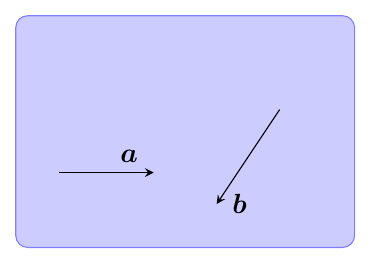
\begin{tikzpicture}[scale=.8,background rectangle/.style={draw=blue!50,fill=blue!20,rounded corners=1ex},show background rectangle]\mystyle
    \clip (0,0)rectangle(5,3.3);
    \draw[myvec](.5,1)--(2,1)node[above left]{$\veca$};
    \draw[myvec](4,2)--(3,.5)node[right]{$\vecb$};
  \end{tikzpicture}
\end{frame}

\begin{frame}{向量减法之共线}
  
  设$\veca$与$\vecb$方向相同,则$|\veca-\vecb|=\big||\veca|-|\vecb|\big|$;

  设$\veca$与$\vecb$方向相反,则$|\veca-\vecb|=|\veca|+|\vecb|$;
\pause\par\vspace*{-1.7in}
  \qquad\includegraphics[width=0.35\textwidth]{d222s1png}\pause\qquad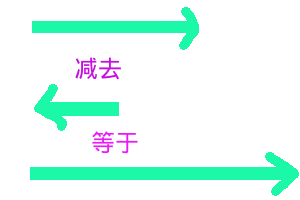
\includegraphics[width=0.35\textwidth]{d222s2.png}
\end{frame}

\begin{frame}{向量减法运算}
  \begin{columns}\begin{column}{.4\textwidth}
  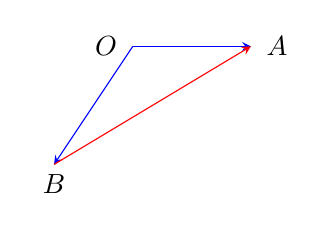
\begin{tikzpicture}<1->\mystyle
    \coordinate[label=left:$O$](O)at(0,0);
    \coordinate[label=right:$A$](A)at(1.5,0);    
    \coordinate[label=below:$B$](B)at(-1,-1.5);
    \draw[myvec,blue](O)--(A);
    \draw[myvec,blue](O)--(B);\pause
    \draw[myvec,red](B)--(A);
  \end{tikzpicture}\end{column}\begin{column}{.6\textwidth}<3->\pause
    \beamercolorlinebox{$\lvec{OA}-\lvec{OB}=\lvec{BA}$\quad 首同尾连指被减}
\end{column}\end{columns}
\end{frame}
 %课本练习第1小题

\begin{frame}{例题}\begin{columns}\begin{column}{.6\textwidth}
  \begin{exampleblock}{找向量}
    如图,在平行四边行$ABCD$中,$\lvec{AB}=\veca,\ \lvec{AD}=\vecb$, 用$\veca,\vecb$表示向量$\textcolor{red!70}{\lvec{AC},\lvec{BD}}$.
  \end{exampleblock}\end{column}\begin{column}{.4\textwidth}
    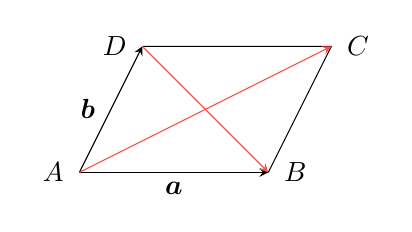
\begin{tikzpicture}[scale=.8]\mystyle
      \coordinate[label=left:$A$](A)at(0,0);
      \coordinate[label=right:$B$](B)at(3,0);    
      \coordinate[label=right:$C$](C)at(4,2);
      \coordinate[label=left:$D$](D)at(1,2);
      \draw[myvec](A)--(B);
      \draw[myvec](A)--(D);
      \draw(B)--(C)--(D);\pause
      \draw[myvec,red!70](A)--(C);\pause
      \draw[myvec,red!70](D)--(B);
      
      \node[left]at(.5,1){$\vecb$};
      \node[below]at(1.5,0){$\veca$};
    \end{tikzpicture}
  \end{column}\end{columns}
\end{frame}

\begin{frame}{例题}
  \begin{exampleblock}{对下列各式进行化简}\setbeamercovered{transparent}
    \begin{enumerate}[<+>]
      \item $\lvec{AB}-\lvec{AC}+\lvec{BD}-\lvec{CD}$
      \item $\lvec{OA}+\lvec{OC}+\lvec{BO}-\lvec{CO}$
    \end{enumerate}
  \end{exampleblock}
\end{frame}


\begin{frame}{例题}\begin{columns}\begin{column}{.6\textwidth}
  \begin{exampleblock}{证明}
    如图,在平行四边行$ABCD$中,$\lvec{AB}=\veca,\ \lvec{DA}=\vecb$, $\lvec{OC}=\vecc$, 证明$\vecb+\vecc-\veca=\lvec{OA}$.
  \end{exampleblock}\end{column}\begin{column}{.4\textwidth}
    \begin{tikzpicture}[scale=.8]
      \coordinate[label=left:$A$](A)at(0,0);
      \coordinate[label=right:$B$](B)at(3,0);    
      \coordinate[label=right:$C$](C)at(4,2);
      \coordinate[label=left:$D$](D)at(1,2);
      \draw[arrows={-stealth[inset=2pt,length=15pt]},red!85](A)--(B);
      \draw[arrows={-stealth[inset=2pt,length=15pt]},red!85](D)--(A);
      \draw[-stealth](A)--(O);
      \draw (D)--(B);
      \draw[-stealth,red!85](O)--(C);
      \draw(B)--(C)--(D);
      \node[left]at(.5,1){$\vecb$};
      \node[below]at(1.5,0){$\veca$};
      \node[below]at(1.5,1){$O$};
      \node[above]at(2,1.3){$\vecc$};
    \end{tikzpicture}
  \end{column}\end{columns}
\end{frame}

\begin{frame}{练习 (这不是最后一道题)}
\setbeamercovered{transparent}
\begin{itemize}[<+>]
\item $\lvec{AB}-\lvec{AD}=\lines$ \\
\item $\lvec{BA}-\lvec{BC}=\lines$ \\
\item $\lvec{AO}-\lvec{BO}=\lines$ \\
\item $\lvec{OB}-\lvec{OC}-\lvec{DB}=\lines$ \\
\item $\lvec{NQ}+\lvec{QP}+\lvec{MN}-\lvec{MP}=\lines$ \\
\item $\big(\lvec{AB}-\lvec{CD}\big)-\big(\lvec{AC}-\lvec{BD}\big)=\lines$ \\
\end{itemize}
%也可以先化为加法来做
\end{frame}

\begin{frame}{推理}
\kaishu
  \begin{columns}
  \begin{column}{0.45\textwidth}
    \begin{block}<1->{向量加法的不等式}
      $\big||\veca|-|\vecb|\big| \le |\veca + \vecb| \le |\veca|+|\vecb|$
    \end{block}
  \end{column}
  \begin{column}{0.55\textwidth}
    \begin{block}<2->{向量减法的不等式}
     向量减法有没有类似的不等式呢?\par\pause
     答:有 (但就是不告诉你)。
    \end{block}
  \end{column}
  \end{columns}
\end{frame}

\begin{frame}{最后一道题}
  若向量$\veca$与$\vecb$满足$|\veca|=5, |\vecb|=12$, 则$|\veca+\vecb|$的最小值是\lines, $|\veca-\vecb|$的最大值是\lines.
\end{frame}

\begin{frame}{小结}
\setbeamercovered{transparent}
\begin{itemize}[<+->]\pause
  \item 减去一个向量被定义为加上它的相反向量
  \item 向量减法口决:首同尾连指被减
  \item $\lvec{OA}-\lvec{OB}=\lvec{BA}$, 化简要点:找相同顶点
  \item $\big||\veca|-|\vecb|\big| \le |\veca\textcolor{red}{\pm}\vecb| \le |\veca|+|\vecb|$
\end{itemize}
\end{frame}

\end{document}

反思:2015.4.1
    这节课有两个主要目标,一个是在图形中找到或作出两个向量的差向量,另一个是在没有图形的情况下化简式子,而我对这两个要点体现的不够,对应的练习也不够,而且练习中还有很多错误,这是备课不充分造成的。
    这次在备课,做课件用去了大多数的时间,没有写教学案。导致的结果是,上课不熟练,在词句之间停顿过多,把语句顺序搞错,而且对于各个环节的连接也处理的不好,总是忘记这个环节处理完之后下一个环节是什么。
    下次备课一定要准备充分,写教学案,反复回忆教学过程,弄熟练;准备更多的习题,准备学生上课可以练习的习题。
    这次上课,由于害怕处理不好,加上不少同学没有听,所以没有让学生上讲台板演,这一点是不好的,以后要学会让学生多动手。
    本打算讲成文质彬彬,有文艺气息的课堂,但是根本就不熟练,所以讲得一点也没有文艺范。下次还是讲成一节实用的课堂吧!
    


